\documentclass{FastFyp}
\usepackage{tikz}
\usetikzlibrary{arrows.meta}
\definecolor{wnavy}{HTML}{1F4E79}
\definecolor{wblue}{HTML}{2E75B6}
\definecolor{worange}{HTML}{C55A11}
\definecolor{wtint}{HTML}{EAF1F8}
% tables: same grid style as the template, set slightly tighter so the report fits in ten pages
\newenvironment{rtab}{\small\singlespacing\renewcommand{\arraystretch}{1.3}}{}
% keep figures next to their text instead of on pages of their own
\renewcommand{\topfraction}{0.9}
\renewcommand{\bottomfraction}{0.8}
\renewcommand{\textfraction}{0.1}
\renewcommand{\floatpagefraction}{0.85}
% references close the last chapter instead of opening a new one
\renewcommand{\bibsection}{\section*{References}}

\begin{document}
\newcommand{\university}{National University of Computer and Emerging Sciences, Lahore}
\newcommand{\fyptitle}{WAF Studio: An Explainable Reverse-Proxy Web Application Firewall}
\newcommand{\Studentone}{Shazil Hamzah}
\newcommand{\Studenttwo}{Nufil Anwar}
\newcommand{\Studentthree}{Muhammad Wahaj}
\newcommand{\Studentfour}{Muhammad Saad}
\date{\today}
\renewcommand{\contentsname}{Table of Contents}

\makeatletter
    \begin{titlepage}
        
\includegraphics[width=0.2\linewidth]{Figures/nulogo.png}\hfill
        
\includegraphics[width=0.2\linewidth]{Figures/fast.png}\\
        \begin{center}
            {\large\bfseries \university}\\[7ex]
            
\includegraphics[width=0.4\linewidth]{Figures/fastlogo.png}\\[8ex]
            {\huge \bfseries \fyptitle }\\[10ex]
            {\Studentone}\\{\Studenttwo}\\{\Studentthree}\\{\Studentfour}\\[10ex]
            {Information Security Project Report}\\
            {Proposal 44, Class 3, Group 12}\\
            {\large \@date}
        \end{center}
    \end{titlepage}
\makeatother
\frontmatter

\pagestyle{empty}
\section*{Abstract}
WAF Studio is a teaching web application firewall, running as a reverse proxy in front of a deliberately vulnerable test shop. It decodes and normalizes every request, matches it against a verified rule language, adds up a score, forwards, flags or blocks the request, and stores the evidence that explains the decision. A role-based browser console provides analysis, reporting, tuning through scoped exceptions and a tamper-evident audit trail. During the final evaluation, the system passed 119 out of 123 mandatory tests, caught 77 of 80 attacks in a controlled corpus and did not have any false positives on 68 benign requests, while adding less than 2~ms per request at the 95th percentile.

\section*{Executive Summary}
Most firewall demonstrations simply demonstrate that a request has been denied. WAF Studio was designed so that a learner can also see \emph{why}: which rules matched, where in the request they matched, what decoding was needed to discover them, and how they added up to the result.

The system has four parts that all listen on 127.0.0.1: an inspecting reverse proxy (port 8080), a security engine shared by the proxy and the console, a role-based console with a JSON API backed by SQLite (port 3000), and a vulnerable test shop with fake data (port 3001). The engine ships with 41 rules, flags a request at a score of 3, blocks it at 5, and is capable of running in a monitor mode that only records. Administrators change versioned rules and configuration; operators ask for very specific exceptions, which a different administrator must approve.

The last acceptance run was successful: all 806 automated tests passed and no known issue was found in the production dependencies. Four attempts to evade the engine by splitting or wrapping a payload are still missed; there are no hidden failures, only reported ones. All results were obtained from a synthetic corpus on a single laptop and cannot be taken as a claim about internet traffic.

\pagestyle{fancy}
\pagebreak
\tableofcontents

\mainmatter

%==================================================================
\chapter{Introduction}
This chapter states the problem, the objectives and scope of the project, and how the work was divided.

\section{Problem Statement}
Web applications are breached through their inputs: SQL injection, cross-site scripting, path traversal and command injection are still prevalent risks as of today \cite{ref:owasptop10}. Production firewalls such as ModSecurity with the OWASP Core Rule Set \cite{ref:modsecurity,ref:crs} can address many of these attacks, but they are difficult to learn from: a blocked request typically returns only a bare 403, and rule files and logs have to be read by hand to understand the decision. The project thus requests a working firewall that can be studied end to end in a closed lab and that explains all of its decisions.

\section{Objectives and Scope}
WAF Studio aims to (i) accept traffic both from a real HTTP proxy and from a console, (ii) explain the decision for every request, (iii) maintain reproducible evidence of each decision, and (iv) safeguard its own users and data. All seven modules called for in the proposal are implemented: request parsing, a rule language, scoring, block and monitor modes, rate limits, an audit console, and tuning with exceptions. Hosting, TLS, external targets and real attack deployment are out of scope.

\section{Team and Work Division}
The work was split into four workstreams (Table~\ref{tab:team}). The system was developed with Claude, an AI coding assistant, as detailed in the log in \texttt{docs/PROGRESS.md}.

\begin{table}[!h]
\centering
\caption{Workstreams and owners.}
\begin{rtab}
\begin{tabular}{|p{3.2cm}|p{10.3cm}|}
\hline
\textbf{Member} & \textbf{Workstream} \\
\hline
Shazil Hamzah (A) & Backend, data and authentication: API, SQLite repositories, sessions, reverse proxy \\
\hline
Nufil Anwar (B) & Security engine and evaluation fixtures: parser, rule language, scoring, 41 rules \\
\hline
Muhammad Wahaj (C) & Frontend, reporting and integration: console, report export, user guide \\
\hline
Muhammad Saad (D) & Automation, security testing and QA: test shop, test suites, evaluation, threat model \\
\hline
\end{tabular}
\end{rtab}
\label{tab:team}
\end{table}

The design and implementation are described in Chapter~2, testing and results in Chapter~3, and conclusions in Chapter~4.

%==================================================================
\chapter{System Design and Implementation}
The architecture, the request pipeline, the engine, the console and the controls that safeguard the application itself are presented in this chapter. The system runs on Node.js 22.13 or newer; its only production dependencies are Express and http-proxy, and storage uses the SQLite module that is native to Node.

\section{System Architecture}
The two paths a request takes to the engine are shown in Figure~\ref{fig:arch}. A user who has signed in uses the console, which calls the API; any HTTP client can instead send traffic to the reverse proxy. Both paths call the same engine with the same active policy, so a request analysed in the console receives the same decision it would get through the proxy. Events, policy versions and the audit chain are stored in SQLite, and allowed requests are forwarded to the test shop. If the shop is down the proxy returns a safe 502; if inspection itself fails the request fails closed with a 503. The block page displays just an event identifier, not the rule that fired.

\begin{figure}[!htb]
\centering
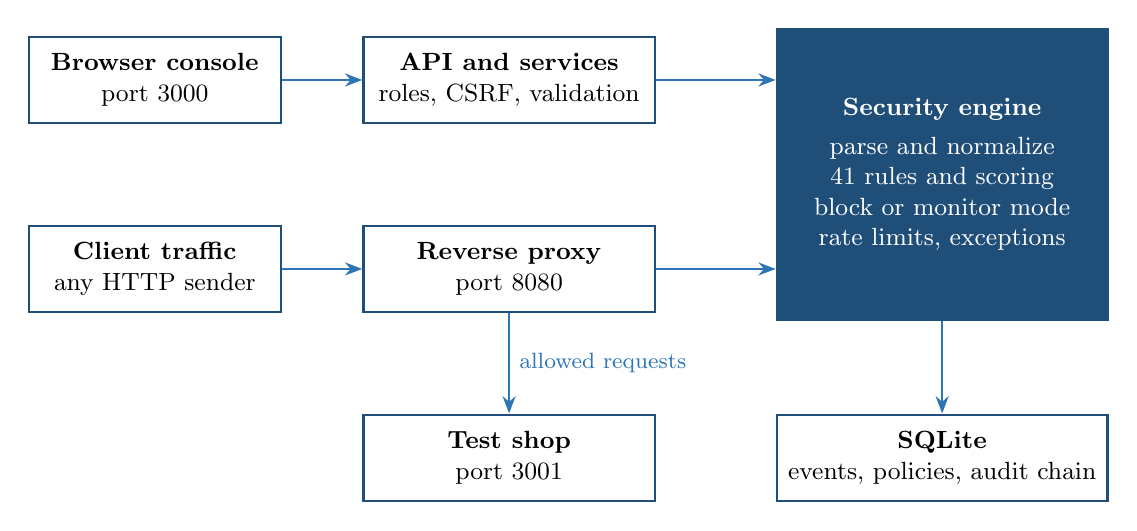
\begin{tikzpicture}[font=\small, >={Stealth[length=2.2mm]},
  box/.style={draw=wnavy, thick, fill=white, align=center, minimum height=1.1cm, text=black},
  big/.style={draw=wnavy, thick, fill=wnavy, align=center, text=white}]
  \node[box, minimum width=3.2cm] (br) at (1.6,3.4) {\textbf{Browser console}\\port 3000};
  \node[box, minimum width=3.7cm] (api) at (6.1,3.4) {\textbf{API and services}\\roles, CSRF, validation};
  \node[box, minimum width=3.2cm] (cl) at (1.6,1.0) {\textbf{Client traffic}\\any HTTP sender};
  \node[box, minimum width=3.7cm] (px) at (6.1,1.0) {\textbf{Reverse proxy}\\port 8080};
  \node[big, minimum width=4.2cm, minimum height=3.7cm] (en) at (11.6,2.2) {\textbf{Security engine}\\[1mm]parse and normalize\\41 rules and scoring\\block or monitor mode\\rate limits, exceptions};
  \node[box, minimum width=3.7cm] (sh) at (6.1,-1.4) {\textbf{Test shop}\\port 3001};
  \node[box, minimum width=4.2cm] (db) at (11.6,-1.4) {\textbf{SQLite}\\events, policies, audit chain};
  \draw[->, thick, wblue] (br) -- (api);
  \draw[->, thick, wblue] (api.east) -- (en.west |- api.east);
  \draw[->, thick, wblue] (cl) -- (px);
  \draw[->, thick, wblue] (px.east) -- (en.west |- px.east);
  \draw[->, thick, wblue] (px) -- node[right, font=\footnotesize] {allowed requests} (sh);
  \draw[->, thick, wblue] (en) -- (db);
\end{tikzpicture}
\caption{The proxy path and the console path share one security engine and one database. The components are shown with their local port; an arrow indicates the direction that requests flow.}
\label{fig:arch}
\end{figure}

\section{Request Pipeline and Security Engine}
All requests go through the six steps shown in Figure~\ref{fig:pipeline}. The parser enforces limits of 4,096 URL characters, 100 headers, 200 arguments and a 1~MiB body, and examines the first 64~KiB. Each value is maintained in multiple normalized forms (repeated URL decoding, \%u escapes, HTML entities, Unicode NFKC, removal of null and invisible characters, SQL comment and whitespace handling), so disguised payloads still match. Every matching rule is counted once and adds its points to the total, together with its location, a short excerpt and the decoding steps that exposed it; parser anomalies contribute to the same total. A total of 3 or 4 flags the request and 5 or more blocks it with a 403. In monitor mode a request that would be blocked is forwarded and the event records the would-be block. Additionally, the proxy limits each client pseudonym to 300 requests per minute.

\begin{figure}[!htb]
\centering
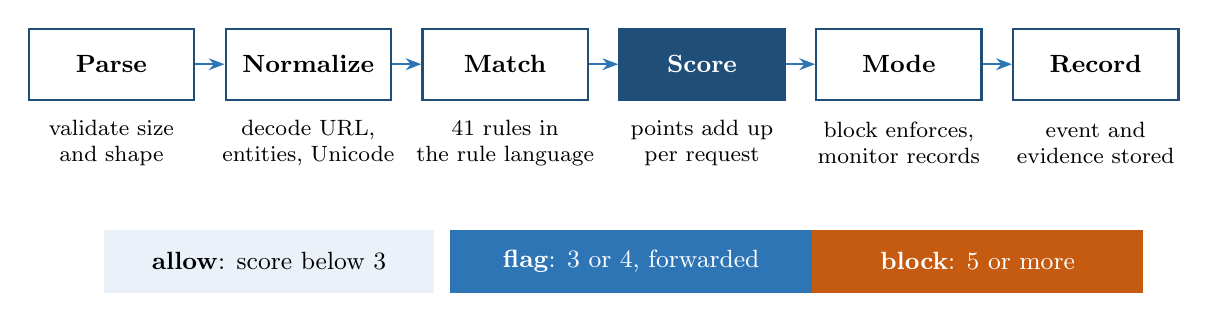
\begin{tikzpicture}[font=\small, >={Stealth[length=2mm]},
  st/.style={draw=wnavy, thick, fill=white, minimum width=2.1cm, minimum height=0.9cm, align=center}]
  \foreach \i/\t/\d in {0/Parse/{validate size\\and shape},1/Normalize/{decode URL,\\entities, Unicode},2/Match/{41 rules in\\the rule language},3/Score/{points add up\\per request},4/Mode/{block enforces,\\monitor records},5/Record/{event and\\evidence stored}} {
    \pgfmathsetmacro{\x}{\i*2.5}
    \ifnum\i=3 \node[st, fill=wnavy, text=white] (n\i) at (\x,0) {\textbf{\t}};
    \else \node[st] (n\i) at (\x,0) {\textbf{\t}}; \fi
    \node[font=\footnotesize, align=center] at (\x,-1.0) {\d};
  }
  \foreach \i/\j in {0/1,1/2,2/3,3/4,4/5} \draw[->, thick, wblue] (n\i) -- (n\j);
  \node[minimum width=4.2cm, minimum height=0.8cm, fill=wtint, align=center] at (2.0,-2.5) {\textbf{allow}: score below 3};
  \node[minimum width=4.6cm, minimum height=0.8cm, fill=wblue, text=white, align=center] at (6.6,-2.5) {\textbf{flag}: 3 or 4, forwarded};
  \node[minimum width=4.2cm, minimum height=0.8cm, fill=worange, text=white, align=center] at (11.0,-2.5) {\textbf{block}: 5 or more};
\end{tikzpicture}
\caption{There are six steps to inspection. In the Score step, the total score determines which of the three outcomes occurs, as indicated in the bottom row.}
\label{fig:pipeline}
\end{figure}

Rules are written in a small language. Invalid rules are rejected with a line and column, rules containing regular expressions that may backtrack catastrophically are refused, and all stored rules are versioned. The 41 default rules include SQL injection (10), cross-site scripting (10), protocol violations (6), path traversal (5), command injection (5) and scanners (5). One rule, with its pattern shortened:

{\small\singlespacing
\begin{verbatim}
rule 942100 "SQLi boolean tautology" {
  when args, cookies matches /\b(?:or|and)\b ... (?:0x[0-9a-f]{1,16}|\d{1,10}) .../i
  severity critical   score 5   category sqli
}
\end{verbatim}}

\section{Console and Roles}
The console is written in pure JavaScript modules without any framework and loads nothing from the network, so a strict Content Security Policy can be applied. The screens are organised by task, and a command menu (Ctrl+K) lets the user reach any action the role allows. The Overview (Figure~\ref{fig:dash}) shows how many requests were inspected, blocked and passed. Opening an event displays all matched rules with their points and location, the score relative to the thresholds, and how to request a scoped exception instead of disabling the rule. Create requests include an idempotency key, which means a request that is retried will not cause a duplicate.

There are three roles, enforced on the server. A \textbf{viewer} is able to see the overview and sanitized event summaries. An \textbf{operator} can also open evidence, compare and replay events, analyse or import samples, request exceptions and export reports. An \textbf{administrator} can also edit rules and configuration, approve exceptions, view the audit log and manage users. An exception is bound to a path prefix, method and location and must be approved by an administrator different from the requester.

\begin{figure}[!htb]
\centering
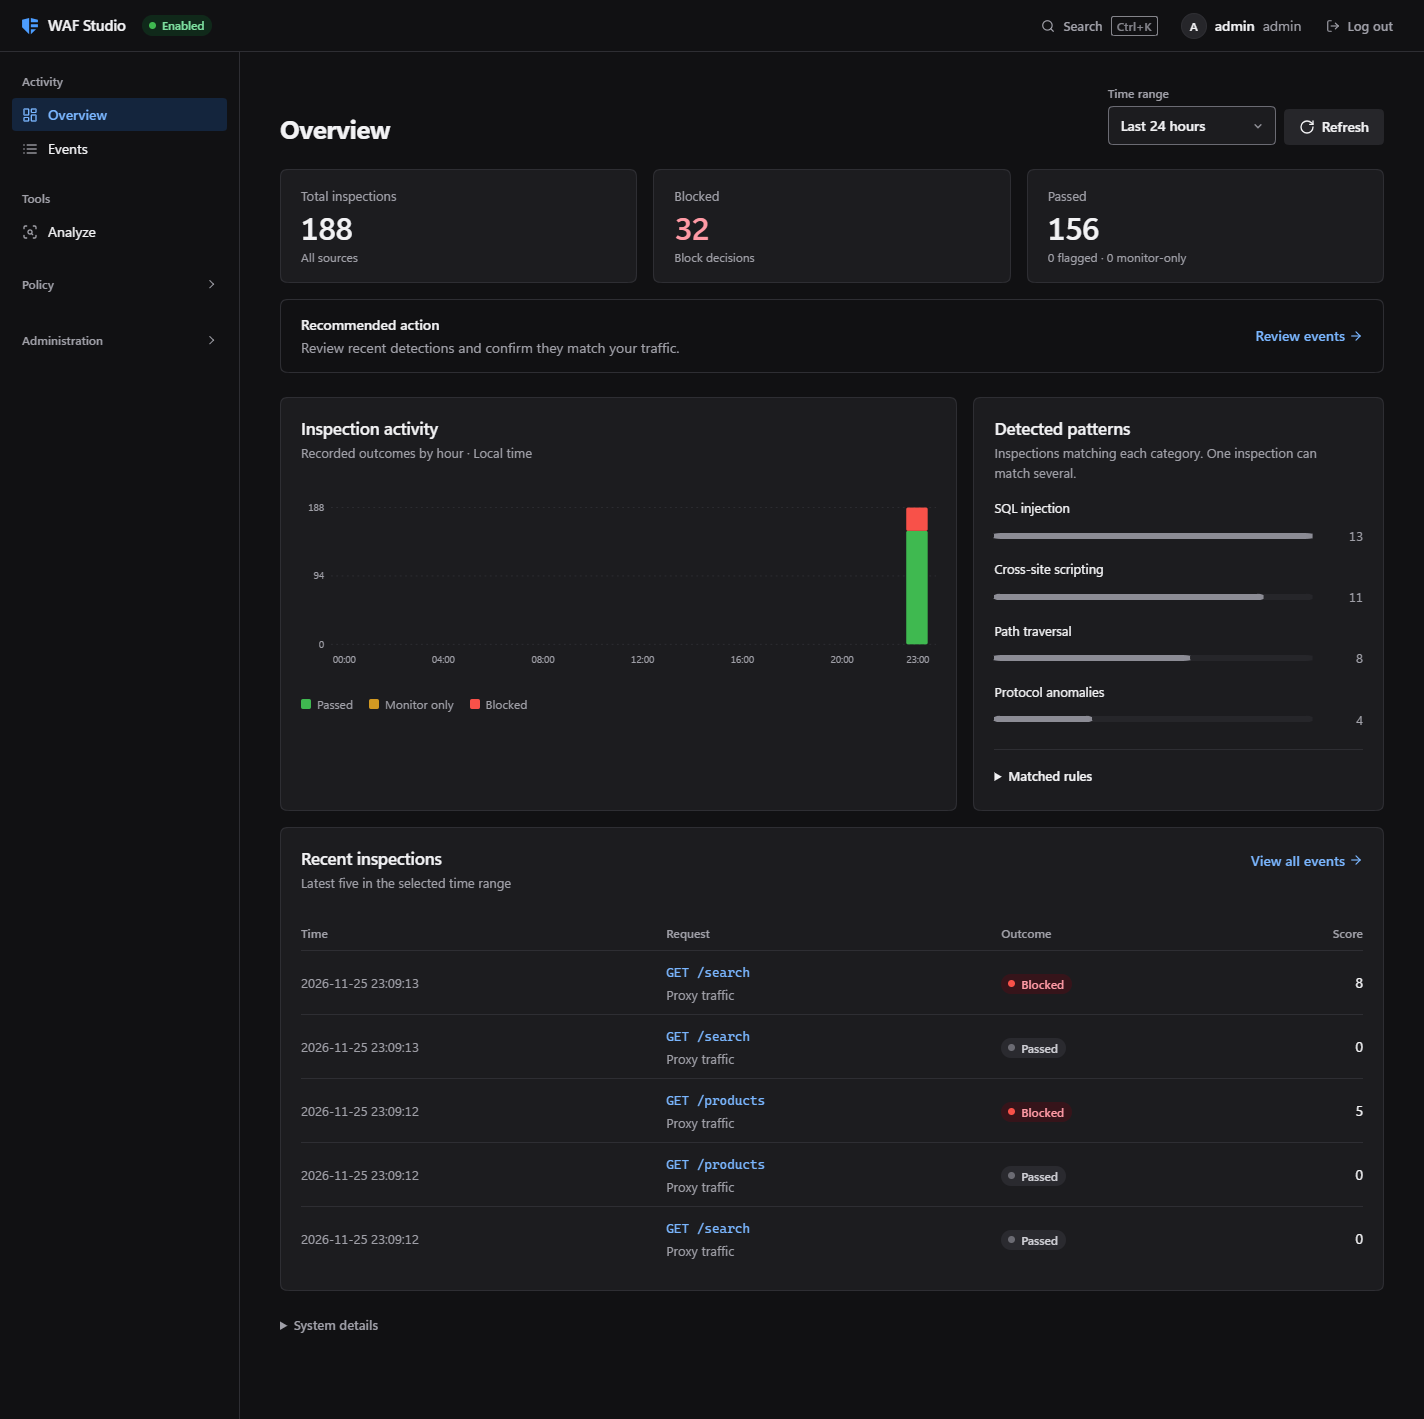
\includegraphics[width=0.72\textwidth, trim=0 600 0 0, clip]{Figures/dashboard.png}
\caption{The Overview screen after running a test of 188 requests: outcome cards, recommended action, hourly activity by outcome and the most common detection categories.}
\label{fig:dash}
\end{figure}

\section{Security of the Application}
The console's own security was treated as a requirement, because the console itself displays attack payloads as evidence. A STRIDE threat model \cite{ref:shostack} includes five trust boundaries and 13 data flows and maps 20 threats to mitigations, code and tests. The main controls are given in Table~\ref{tab:controls}.

\begin{table}[!htb]
\centering
\caption{The main security controls in the application and what each one stops.}
\begin{rtab}
\begin{tabular}{|p{7.0cm}|p{6.5cm}|}
\hline
\textbf{Control} & \textbf{What it prevents} \\
\hline
Server-enforced roles, separation of duties & A viewer or operator reaching admin actions \\
\hline
scrypt password hashes, hashed session tokens, CSRF tokens, 30-minute idle and 8-hour absolute expiry & Use of stolen database contents, session reuse, forged requests \\
\hline
Parameterized SQL and strict input schemas & Injection into the application's own database \\
\hline
Text-only DOM construction and strict CSP & Attack samples running inside the console \\
\hline
Redaction and HMAC client pseudonyms & Secrets and raw IP addresses in stored evidence \\
\hline
Append-only, hash-chained audit log & Unnoticed edits to the record \\
\hline
\end{tabular}
\end{rtab}
\label{tab:controls}
\end{table}

%==================================================================
\chapter{Testing and Results}
This chapter describes the testing procedure for the system and the results obtained.

\section{Method}
The evaluation begins with the full stack running on temporary localhost ports with a fresh database, sends fixture requests through the real proxy to the test shop, and then reads each stored event back via the API. Expected outcomes were set as protection goals before measurement; if an evasion is not blocked, its expected ``block'' is not changed and it is counted as a failure. The runs used Node v24.19.0 on Windows with an Intel Core Ultra 7 255H (16 logical processors), engine 1.0.0 and the default thresholds. Separately, the strict acceptance run passed \textbf{806 of 806} automated tests in 39 suites, and \texttt{npm audit} found no vulnerabilities in the production dependencies.

\section{Mandatory Cases}
Of the 123 mandatory checks, 119 passed (Table~\ref{tab:cases}). Two evasion cases were fixed during the project, a hexadecimal tautology and a \texttt{||}-concatenated tautology; both are now blocked, and unit and end-to-end tests confirm that benign look-alikes still pass.

\begin{table}[!htb]
\centering
\caption{The mandatory evaluation cases and results.}
\begin{rtab}
\begin{tabular}{|p{6.2cm}|p{2.6cm}|p{4.7cm}|}
\hline
\textbf{Case} & \textbf{Passed} & \textbf{Note} \\
\hline
T1 Injection strings (SQLi, XSS, traversal) & 28 of 28 & All blocked \\
\hline
T2 Encoding and normalization variants & 20 of 20 & All blocked \\
\hline
T3 Difficult benign inputs & 38 of 38 & All allowed \\
\hline
T4 Large bodies and size limits & 6 of 6 & Inspection window observed \\
\hline
T5 Evasion attempts & 14 of 18 & Four misses kept as failures \\
\hline
T6 Latency overhead & 2 of 2 & Below 25 ms \\
\hline
T-final Failure, denial and restart & 11 of 11 & Safe behaviour, state persisted \\
\hline
\textbf{Total} & \textbf{119 of 123} & \textbf{96.7\%} \\
\hline
\end{tabular}
\end{rtab}
\label{tab:cases}
\end{table}

\section{Detection and Latency}
A separate set of 80 attacks and 68 benign requests resulted in 77 true positives, 3 false negatives, 68 true negatives and no false positives: precision 1.00, recall 0.9625 and F1 0.981. Figure~\ref{fig:cov} shows coverage by category. The engine took 0.126~ms at the median and 0.277~ms at the 95th percentile. In the latency benchmark (300 interleaved request pairs per scenario after 30 warm-ups) the proxy added 1.721~ms to a GET and 1.886~ms to a 2~KiB form POST at the 95th percentile (Table~\ref{tab:latency}), with no failed requests.

\begin{figure}[!htb]
\centering
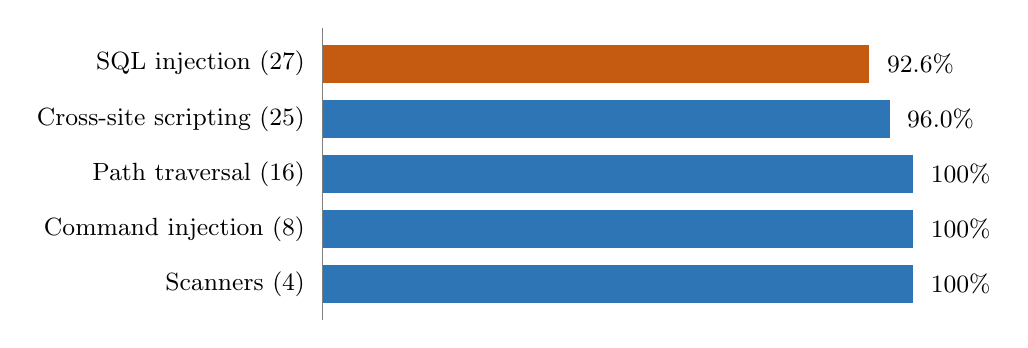
\begin{tikzpicture}[font=\small]
  \foreach \i/\n/\v/\c in {0/{SQL injection (27)}/92.6/worange, 1/{Cross-site scripting (25)}/96.0/wblue, 2/{Path traversal (16)}/100/wblue, 3/{Command injection (8)}/100/wblue, 4/{Scanners (4)}/100/wblue} {
    \pgfmathsetmacro{\y}{-\i*0.7}
    \pgfmathsetmacro{\w}{\v*0.075}
    \node[anchor=east] at (0,\y) {\n};
    \fill[\c] (0.1,\y-0.24) rectangle (0.1+\w,\y+0.24);
    \node[anchor=west] at (0.2+\w,\y) {\v\%};
  }
  \draw[gray] (0.1,0.45) -- (0.1,-3.25);
\end{tikzpicture}
\caption{The percentage of corpus attacks found in each category (number of attack samples in brackets). Two of the three remaining split-payload misses are in the top bar, SQL injection.}
\label{fig:cov}
\end{figure}

\begin{table}[!htb]
\centering
\caption{Response time at the 95th percentile, in milliseconds.}
\begin{rtab}
\begin{tabular}{|p{4.2cm}|p{2.4cm}|p{2.9cm}|p{2.4cm}|}
\hline
\textbf{Scenario} & \textbf{Direct} & \textbf{Through WAF} & \textbf{Added} \\
\hline
GET search & 0.317 & 2.038 & 1.721 \\
\hline
POST 2 KiB form & 0.238 & 2.124 & 1.886 \\
\hline
\end{tabular}
\end{rtab}
\label{tab:latency}
\end{table}

%==================================================================
\chapter{Conclusions}
This chapter outlines the existing limitations and wraps up the report.

\section{Limitations}
Four attempts at evasion are still not caught: SQL tokens split across query parameters, SQL tokens split across JSON fields, base64-wrapped markup, and markup split across duplicate parameters. Matching each value alone cannot reconstruct a payload that is only assembled by the application. Other limits are the 64~KiB inspection window, a heuristic regular-expression guard, in-memory rate-limit windows, no response inspection, no TLS on the loopback interface, and an audit chain that is not anchored outside the database. The corpus is small and shares signature families with the tests, so the figures describe behaviour in this lab only.

\section{Conclusion and Future Work}
WAF Studio fulfils the goals of the proposal. It makes explainable decisions through both a reverse proxy and a console, supports safe tuning with two-person approval of exceptions, keeps tamper-evident evidence, and ensures the security of its own users and data, while reporting its misses openly. Future work could include cross-parameter reconstruction for split payloads, response inspection, TLS termination, an externally anchored audit chain and an independent test corpus.

{
\bibliographystyle{ieeetr}
\bibliography{fypbib}
}

\end{document}
